\section{Factories\label{Factory}}
\subsection{Origineel}
Bij de creatie van domein-specifieke objecten moeten er verschillende objecten gemaakt worden van dezelfde familie maar met verschillende attributen. 
Daarom werd er gekozen voor een factory-method patroon. 
Aangezien dit generisch werd gedaan, werden de factory-methodes geabstraheerd naar elk hun eigen klasse. 
De lijst met attributen is dan aangepast naar een generische lijst van Argument's. 
Dit is een object dat een vraag en het verwachte type encapsuleert en de antwoorden interpreteert.\\

Dit werd ook gebruikt bij de resultaten van medische testen en behandelingen: 
de methode $Argument[]\ getEmptyArguments()$ geeft een lijst van informatie die ingevuld moet worden.
Het is dan aan de gebruiker om deze in te vullen met $Argument.enterAnswer(String\ ans)$. 
Bij ieder argument is er een vraag bij gesteld om de gebruiker te tonen welke invoer verwacht wordt. 
Uiteindelijk roept de UI de methode $enterResults(Argument[]\ args)$ aan om de resultaten in te vullen. 

\subsection{Problemen}
Die aanpak introduceerde onnodige complexiteit in het project. 
Ook was het originele patroon van de factory-method niet meer herkenbaar en trad er naamsverwarring op. 
Sommige verantwoordelijkheden die de factory-methodes hadden, werden verkeerdelijk toegekend aan de Controller. 
Zoals de gemaakte medische testen toevoegen bij de patient, en deze inplannen. \\

Bij het invoeren van resultaten waren er geen verantwoordelijkheden verkeerd toegekend, dit systeem is hier dus behouden. 
Als men dit ook wil aanpassen dan moet men op één of andere manier het type van de medische testen bepalen om te kunnen differentiëren. 

\subsection{Aanpassingen}
Het generisch zijn werd verwijderd ten voordele van een "puur" patroon. 
Hierdoor verdwijnt veel van de onnodige complexiteit.
De verkeerde verantwoordelijkheden die aan de Controllers toegekend waren, zijn naar de factory-methods verplaatst.
De koppeling is hetzelfde gebleven, de cohesie is een stukje lager. 
De verantwoordelijkheden zijn nu beter toegekend en het subsysteem werkt overzichtelijker. 
Dit zijn enkele methodes die nu in de Controllers voorzien zijn:

\[ String\ makeBloodAnalysis(String\ focus,\ int\ numberOfImages,\ Priority\ p)\]
\[ String\ makeMachine(String\ type,\ String\ id,\ Location\ location,\ CampusInfo\ info)\]

\subsection{Volledig Design}
In figuur \ref{fig:makeUltraSound} kan een interactiediagramma gevonden worden van de creatie van een nieuwe medische test. 
Deze aanpassingen werden gemaakt voor alle klassen die de interface Factory implementeerden. 
Dit waren alle Factory's die machines aanmaken, die personen aanmaken. 
Ook werden alle Factory's voor medische testen en behandelingen herwerkt. 
Door het gebruik van de factory-methodes is de verantwoordelijkheid van de creatie en de consistent houden van het systeem toegekend aan een specifiek object met een hoge cohesie.
Ook maken de Controllers geen deel meer uit van het systeem zelf, maar bedien ze een API aan de UI aan. 

Voor alle klassen is een factory-method patroon gebruikt, behalve voor machines is er een abstract-factory patroon gebruikt omdat alle signaturen hetzelfde zijn. 
Hierdoor cohesie groter door de machines zelf verantwoordelijk te maken voor hun eigen creatie en consistentie. 
Ook is de uitbreidbaarheid hier groter.
De machines hebben zelf heel weinig verantwoordelijkheden, er is dus geen gevaar dat deze klassen te veel verantwoordelijkheden krijgen. 
Indien de machines later meer verantwoordelijkheden krijgen, of andere attributen kan er nog steeds eenvoudig gekozen worden voor een factory-method patroon.

\begin{figure}

\hspace{-2.5cm}
 \includegraphics[width=1.3\textwidth]{./exported/interaction/makeUtraSound.pdf}
 % makeUtraSound.pdf: 1690x520 pixel, 72dpi, 59.62x18.34 cm, bb=0 0 1690 520
\caption{De creatie van een UltraSoundScan medische test \label{fig:makeUltraSound}}

\end{figure} 

\subsection{Uitbreidbaarheid}
Indien er een nieuw user-type,een nieuw machine-type,een nieuw type medische test of een nieuwe behandeling wordt aangemaakt, moeten de nodige klassen aangemaakt worden. 
Er moet ook per type (of per klasse) een nieuwe factory-methode aangemaakt worden en een nieuwe Controller-methode die de creatie van dat type object toelaat aan de UI.
De UI moet ook een passend invoer-menu krijgen. 
Ondanks het feit dat het werk om een nieuw type te maken een beetje groter is dan het vorige design, is de uitbreidbaarheid ook groter. \\

Ook is het design onderhoudbaarder: de informatie moet niet meer door juist één type klasse bijgehouden worden. 
Indien er een grote uitzondering is voor een bepaald type dan is deze, omdat er een aparte methode is, veel gemakkelijker aanpasbaar.
Het is wel nadelig dat voor een nieuw type verschillende methodes moeten bijgemaakt worden. 
Indien er 20 types medische testen zijn dan kan het overzicht door de hoeveelheid code verdwijnen.\\

Dit is misschien meer werk om een eenvoudig object toe te voegen.
Maar indien een soort uitzondering nodig is, dan moet er geen nieuw Argument-type aangemaakt worden. 
Bijvoorbeeld een object die data nodig heeft die niet direct beschikbaar is, zou in het vorige design een nieuw type Argument nodig hebben. 

\subsection{Voorbeeld\label{sec:factVB}}
In figuur \ref{fig:makeUltraSound} kan men zien hoe zo'n factory-method werkt. 
Hier wordt een nieuwe medische test (UltraSoundScan) aangemaakt voor een bepaalde patiënt(Patient).
Voor behandelingen, personen en machines werkt dit analoog. 
De Controller wordt aangeroepen met de nodige parameters: de informatie die nodig is voor die medische test. \\

De Controller delegeert de oproep aan de juiste factory-methode. 
Deze maakt de medische test aan en laat deze dan afhandelen door de $handleCorrectness$ methode, zoals alle andere medische testen. 
Het afhandelen werd vroeger in de Controller zelf gedaan. \\
%Dit was een verkeerde verantwoordelijkheid want de Controllers mogen normaal geen code bevatten die de correctheid van het systeem moet garanderen.\\

De $handleCorrectness$ methode heeft de verantwoordelijkheid om de medische testen juist in de wereld (World) toe te voegen. 
Er wordt een MedicalTestCommand aangemaakt met de medische test die moet toegevoegd worden en deze wordt toegevoegd aan de geschiedenis van de dokter(Doctor) die deze aanmaakt. 
Tijdens het toevoegen wordt deze ook uitgevoerd. 
Het uitvoeren en ongedaanmaken van commando's is nu de verantwoordelijkheid van de CommandHistory-klasse.
Dit was vroeger ook de verantwoordelijkheid van de Controllers. 
Het probleem was dus dat er Commando's konden toegevoegd worden aan de lijst van uitgevoerde Commando's zonder dat deze uitgevoerd waren.


\section{Scheduling\label{scheduling}}
\subsection{TimeFrameConstraint}
\subsubsection{Origineel}
Het originele design van de TimeFrameConstraints\footnote{De naam van deze klasse is voor de duidelijkheid behouden, een betere naam is AppointmentConstraint of Constraint} kan men zien op figuur \ref{fig:constraints_old}. 
Men kan duidelijk zien dat de ``hulp''-hiërarchie die bepaalde hulp-methodes instantieert nodeloos complex is.\\

Een ander probleem is dat de beslissing binair is: men kan ofwel de afspraak aanvaarden of niet.
Dit heeft twee sterke nadelen: als de eerst mogelijke afspraak ver weg is, kan dit lang duren indien iedere minuut/ iedere seconde voor een heel jaar overlopen wordt. 
Het andere nadeel is dat er geen enkele controle is die de berekening stopt indien er nooit een afspraak kan gemaakt worden. 
Eén van de voordelen is wel dat nog alle vrijheid behouden wordt om nieuwe Constraints te maken. 
Bij een aangepast design zou dit behouden moeten worden.

\begin{figure}
\vspace{-2cm}
  \begin{center}
    \includegraphics[width=1.0\textheight,angle=270]{./exported/Constraints_OLD.pdf}
    % Constraints_OLD.pdf: 2390x1220 pixel, 72dpi, 84.31x43.04 cm, bb=0 0 2390 1220
  \end{center}
\caption{De oude hiërarchie van TimeFrameConstraints\label{fig:constraints_old}}
\vspace{2cm}
\end{figure} 

\subsubsection{Aanpassingen}
Het nieuwe design van de TimeFrameConstraints kan men zien in figuur \ref{fig:Constraints}. 
Hier is de hierarchie verwijderd en blijft enkel een interface over die de nodige methodes aanbiedt. 
Een nieuwe Constraint maken is dus eenvoudiger. 
Ook de gelinkte structuur is gewisseld voor een lijst, waardoor de grootste complexiteit verdwenen is. \\

De beslissing of een Constraint aanvaard wordt of niet wordt nu gedaan door een Time object terug te geven. 
Dit is het eerstvolgende moment waarop deze constraint aanvaard kan worden. 
Indien de huidige tijd aanvaard wordt, wordt de huidige tijd bevestigd. 
Indien er een probleem is, wordt een ScheduleException gegooid. \\

De tijd die teruggegeven wordt, moet een conservatieve schatting zijn. 
Dit wil zeggen dat indien er mogelijks momenten zijn die onzeker zijn, mag men deze niet overslaan. 
Desnoods stapt men naar de volgende minuut zoals in het vorige design. 
Met deze aanpassing is er bij een goede implementatie van de meeste constraints geen probleem meer met een lange rekentijd. 
Indien alle Constraints terug de volgende minuut teruggeven zal er natuurlijk geen tijdswinst zijn. 
\begin{figure}
\vspace{-2cm}
  \begin{center}
    \includegraphics[width=1.0\textheight,angle=270]{./exported/Constraints.pdf}
    % Constraints.pdf: 1960x1130 pixel, 72dpi, 69.14x39.86 cm, bb=0 0 1960 1130
  \end{center}
  \caption{Het nieuwe design van de Constraints\label{fig:Constraints}}
\vspace{2cm}
\end{figure} 

\subsection{Voorbeeld}
Figuur \ref{fig:PriorityConstraint} toont hoe de PriorityConstraint werkt. Dit is een typische TimeFrameConstraint. 
Een TimeFrameConstraint wordt bezocht door iedere aanwezige als ieder type in zijn hierarchie om te beslissen of een bepaald moment in orde is. 
Bij een PriorityConstraint worden alle agenda's van de aanwezigen onthouden. 
Wanneer de $isAccepted()$-methode aangeroepen wordt, kijkt deze voor iedere agenda alle afspraken op hetzelfde moment na of deze een hogere prioriteit hebben. 
Indien er een conflict is dan is de eindtijd van de afspraak het eerstvolgende moment die getest zal worden. \\

Andere TimeFrameConstraints werken analoog: ze worden bezocht door de aanwezigen, ze vragen de nodige informatie op en maken aan de hand daarvan een beslissing. 
PreferenceConstraint, de Constraint die bepaalt hoe een dokter tussen de campussen beweegt, vraagt de preferentie op aan de Doctor en laat de beslissing dan over aan de Preference-interface. 
Door het polymorfisme is het normaal niet meer nodig om de Constraint aan te passen voor nieuwe preferentie-types.

\begin{figure}
  \begin{center}
    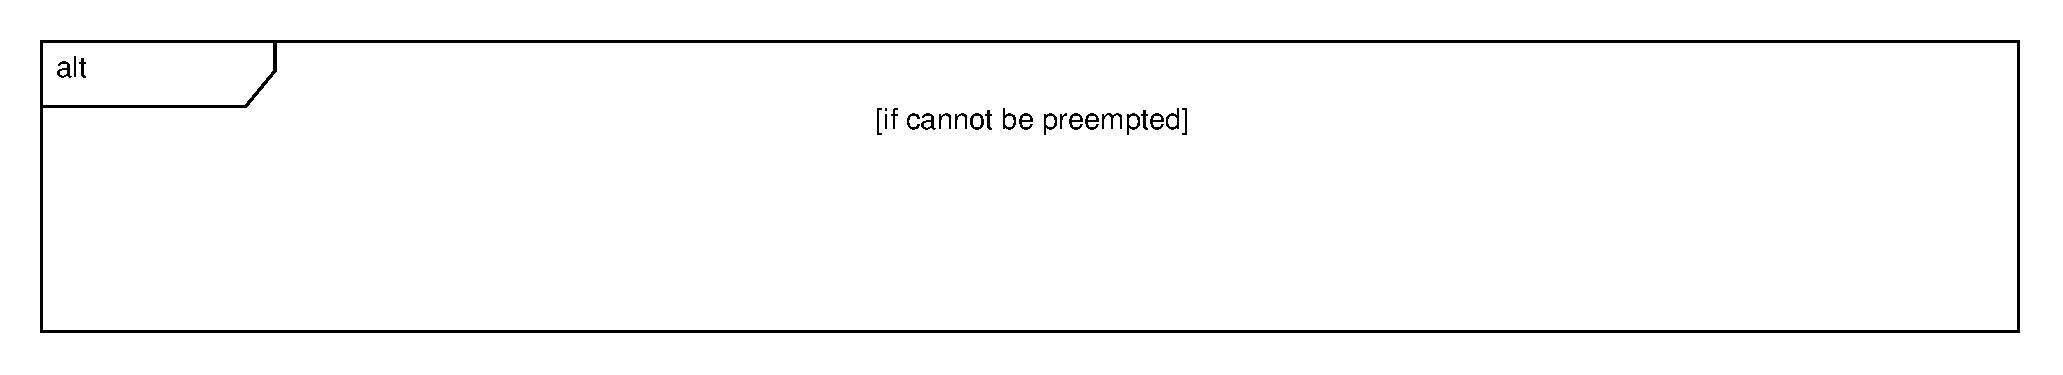
\includegraphics[width=0.7\textwidth]{./exported/interaction/PriorityConstraint.pdf}
    % PriorityConstraint.pdf: 890x690 pixel, 72dpi, 31.40x24.34 cm, bb=0 0 890 690
  \end{center}
\vspace{-1cm}
  \caption{Het interactiediagramma van PriorityConstraint\label{fig:PriorityConstraint}}
\end{figure} 


\subsection{CampusDecider}
\subsubsection{Probleem}
Deze interface breidde de interface van TimeFrameConstraint uit om de Campus te bepalen. 
De interface Appointable gaf een lijst van TimeFrameConstraints terug met als eerste constraint een GetCampusConstraint die de Campus moest bepalen. 
Klassen die deze interface implementeerden hadden een dubbele verantwoordelijkheid: 
de Campus bepalen en hun Constraint evalueren. Dit ging tegen Responsibility-driven design in en dit verlaagt de cohesie en verhoogt de koppeling.

\subsubsection{Aanpasssing}
De interface werd losgekoppeld van de TimeFrameConstraint-interface. 
De TimeFrameConstraint-interface heeft een nieuwe methode $setCampus(Campus c)$. 
Een Appointable heeft hier nu een aparte methode voor die de implementatie hiervan kiest. 
De verantwoordelijkheden van het bepalen van de Campus hoort nu toe aan een nieuwe CampusDecider-klasse.
Appointable bepaalt hoe de Campus beslist wordt(NurseDecides, PatientDecides) en dit object wordt doorgegeven aan de AppointmentConstraintSolver. 

\subsubsection{Voorbeeld}
Medische testen en behandelingen zijn altijd op de campus van de verpleegster die deze toedient (figuur \ref{fig:nurseDecides}). 
Wanneer het NurseDecides object bezocht wordt door een verpleegster, wordt de Campus opgevraagd en opgeslagen. 
Dit is dan de besliste Campus. Dit gebeurt analoog bij een PatientDecides: de patiënt beslist hier en het object onthoudt de Campus van de patiënt.

\begin{figure}
 \centering
 \includegraphics[width=0.7\textwidth]{./exported/interaction/nurseDecides.pdf}
 % nurseDecides.pdf: 800x310 pixel, 72dpi, 28.22x10.94 cm, bb=0 0 800 310
 \caption{Hoe een CampusDecider werkt\label{fig:nurseDecides}}
\end{figure}

\subsubsection{Uitbreidingen}
Het is niet moeilijk om andere beslissingsmethodes te implementeren. 
Men kan eventueel beslissen aan de hand van een voorkeurs Campus, waarbij de meerderheid wint. 
Of aan de hand van bepaalde heuristieken, zoals minimale verplaatsingstijd.
Het is wel nodig dat alle informatie beschikbaar is.

\subsection{TimeFrame}
\subsubsection{Probleem}
De klasse TimeFrame wordt gebruikt om een Time-object en een lengte te combineren. 
De enige reden dat deze klasse bestond is omdat Java maar één return-type ondersteunt. 
Aangezien deze op te veel plaatsen gebruikt werd, was zowel de koppeling met deze klasse hoger als de cohesie hierdoor lager. 

\subsubsection{Aanpassingen}
In de eerste fase van het nieuwe design waren de plaatsen waar dit object voor zijn originele reden gebruikt werd bijna verdwenen. 
Deze klasse is hernoemd naar een AppointmentResult en bezit alle informatie van een geldige afspraak. 
Op de plaatsen waar dit niet van toepassing was, is de TimeFrame opgesplitst in zijn twee delen: Time en lengte.

\subsubsection{Voordelen}
Dit vergroot de duidelijkheid en de eenvoud van dit subsysteem, vooral bij de TimeFrameConstraint-interface. 
De code zelf is ook simpeler en leesbaarder. 

\subsection{AppointmentConstraintSolver en AppointmentCommand}
Deze klassen waren sterk gekoppeld met elkaar. 
Aangezien deze alletwee een grote verantwoordelijkheid hebben, zijn deze instabieler en worden deze best zo veel mogelijk losgekoppeld. 
De klasse SolverAdapter bepaalt nu de communicatie tussen deze klassen met een enkele methode $solve(...)$. 
Deze maakt een AppointmentResult, deze kan rechtstreeks doorgegeven worden aan de constructor van Appointment zodat de koppeling tussen AppointmentConstraintSolver en AppointmentCommand nog meer daalt. 

\subsection{JumpSolver}
Deze klasse is een herschrijving van BruteForceSolver. 
Door de aanpassingen van TimeFrameConstraint kan deze nu sneller een afpsraak maken. 
Men kan nooit alle infinte loops herkennen voor een bepaalde verzameling van aanwezigen, desnoods stopt men met het zoeken na een redelijke tijd.
Dit kan met de huidige verzameling van Constraints ook niet voorkomen: ofwel herkennen ze direct dat ze nooit zullen voldoen, ofwel is er op een lege dag altijd de mogelijkheid om de afspraak te plannen.

\subsection{Volledig Design}
De klassediagrammas in figuren \ref{fig:Constraints}, \ref{fig:fullScheduling} en de interactieschemas in \ref{fig:solver} en \ref{fig:cartesian} tonen het volledige design van het scheduling subsysteem. 
Figuur \ref{fig:Constraints} toont aan van welke klassen de Constraints informatie halen. 
Het andere klassediagramma (figuur \ref{fig:fullScheduling}) toont welke informatie nodig is om een afspraak te kunnen maken. 
De AppointmentCommand verzamelt de CampusDecider, de DelayedTimeLength, alle Constraints en alle ScheduleGroup's. 
Door gebruik te maken van de $solve(...)$ methode wordt een AppointmentResult gegenereerd die gebruikt wordt door het AppointmentCommand om een Appointment te instantieren. 
%Een interactiediagramma hiervan vind je in figuur \ref{fig: AppCreation}.
%TODO
\\

\begin{figure}
\vspace{-2cm}
\centering
 \includegraphics[width=1.05\textheight, angle=270]{./exported/ScheduleGroup_End.pdf}
 % ScheduleGroup End.pdf: 2350x880 pixel, 72dpi, 82.90x31.04 cm, bb=0 0 2350 880
 \caption{The full scheduling subsystem.}
 \label{fig:fullScheduling}
\vspace{2cm}
\end{figure}

\begin{figure}
\hspace{-2cm}
 \includegraphics[width=1.2\textwidth]{./exported/interaction/Solver.pdf}
 % Solver.pdf: 1080x590 pixel, 72dpi, 38.10x20.81 cm, bb=0 0 1080 590
 \caption{Step 1 of the solver}
 \label{fig:solver}
\hspace{2cm}
\end{figure}

\begin{figure}
\hspace{-2cm}
 \includegraphics[width=1.2\textwidth]{./exported/interaction/cartesianProduct.pdf}
 % cartesianProduct.pdf: 1480x820 pixel, 72dpi, 52.21x28.93 cm, bb=0 0 1480 820
 \caption{Step 2 of the solver}
 \label{fig:cartesian}
\end{figure}


De AppointmentConstraintSolver(solver) werkt als volgt: eerst worden alle combinaties van personen gemaakt die nodig zijn voor de afspraak, één per ScheduleGroup. 
Daarna wordt voor iedere combinatie het eerste moment berekend dat er een afspraak kan gemaakt worden, dit gebeurt in schema \ref{fig:solver}. 
Het vroegste moment wordt onthouden en uiteindelijk gebruikt. 
Om de uitbreidbaarheid zo groot mogelijk te houden is er een afscheiding gemaakt tussen zij die aanwezig kunnen zijn, en waar deze informatie opgeslagen is. 
Hierdoor is de koppeling tussen belangrijke systemen tot een minimum herleid en is de cohesie hoger:
de solver heeft geen enkele informatie nodig om een afspraak te plannen.\\

Het berekenen van de eerstvolgende afspraak voor een bepaalde combinatie gebeurt als volgt: alle TimeFrameConstraints worden opgevraagd: van de Appointable, en alle aanwezigen. 
Daarna bezoeken alle aanwezigen de CampusDecider, die de plaats bepaalt.
Als laatste voorbereidingsstap worden alle TimeFrameConstraints bezocht door alle aanwezigen en de Campus.
Dit is de bovenste helft van diagramma \ref{fig:cartesian}. 
Dit design is om dezelfde redenen gekozen als de ScheduleGroup interface, dezelfde GRASP-principes zijn van toepassing. \\

De eerst mogelijke tijd dat een afspraak mag gebeuren, een medische test heeft bijvoorbeeld een vertraging van één uur, wordt opgevraagd. 
Vanaf dan worden de TimeFrameConstraints de tijd en de lengte van de mogelijke afspraak aangeboden en wordt de afspraak iedere keer uitgesteld tot alle TimeFrameConstraints akkoord zijn. 
Vooral het gebruik van polymorfisme laat hier toe om de cohesie van de solver en de Constraints hoog te houden. 
Door het gebruik van de TimeFrameConstraints kunnen verschillende aanwezigen elk hun eigen informatie op een veilige manier delen. 
Op basis hiervan is de koppeling tussen de solver en de domeinlaag veel kleiner. 
De klassen die de interface Schedulable implementeren mogen niet rechtstreeks aangesproken worden in de solver. 
Hierdoor is de solver beschermd tegen veranderingen in de minder stabiele domein-laag.

\subsection{Voorbeeld}
Stel dat er een afspraak moet gemaakt worden voor een Patient p die een XRayScan moet krijgen. 
Er is op elke Campus één XRayMachine en op elke Campus is er één verpleegster. 
Dan wordt een afpsraak op de volgende manier gepland. 
De klasse AppointmentCommand verzamelt de CampusDecider en de Constraints van de medische test, dit is een NurseDecides object en een lijst met een NurseBackToBackConstraint en een XRayConstraint.
Een PriorityConstraint wordt toegevoegd door de AppointmentCommand.
Ook worden alle ScheduleGroup's verzameld: een groep met de Patient p die aanwezig moet zijn en twee MultiSchedulableGroup's voor de aanwezigheid van een Nurse en een XRayMachine. \\

De solver creëert dan alle combinaties van aanwezigen. Dit zijn er hier 4 combinaties van 3 aanwezigen (de patient, een verpleegster en een machine): iedere Patient, Nurse en XRayMachine wordt gecombineerd. 
Dan wordt voor iedere combinatie de Campus bepaald, dit is de Campus van de Nurse. 
Ook worden alle Constraints van de aanwezigen opgevraagd: een Machine kan niet bewegen, een Nurse kan niet bewegen, een Nurse werkt tussen 9u en 17u. \\

Dan wordt er voor iedere combinatie het eerste mogelijke moment berekend dat een afspraak mogelijk is. 
Voor 2 van de 4 combinaties is dit niet mogelijk, de UnmovableConstraint van de XRayMachine zal een SchedulingException gooien en deze berekening zal stoppen. 
Voor de twee andere combinaties zal er uiteindelijk een afspraak gevonden worden die aan alle voorwaarden voldoet. 
De vroegste wordt gekozen als uitkomst, alle nodige informatie wordt opgeslagen.



\section{Aangepaste Use Cases\label{Volledig}}

\subsection{Order MedicalTest\label{use:Med}}
Door aanpassingen aan de creatie van domein-specifieke objecten kan de UI geen lijst van objecten meer opvragen. 
Deze lijst is nu ingebouwd in de UI. 
Bij de start van deze use case wordt aan de gebruiker gevraagd welke medische test hij/zij wil maken. 
Dan wordt de nodige informatie gevraagd aan de gebruiker. De types en vragen zijn ook ingebouwd in de UI.
Uiteindelijk wordt de juiste $make$ methode aangeroepen in de Controller. 
Dit is ook te zien in diagramma \ref{fig:makeUltraSound}, de interne werking werd beschreven in \ref{sec:factVB}.

\subsection{Enter Diagnosis}
Bij het begin van deze use case wordt er aan de gebruiker gevraagd of deze diagnose een tweede opinie nodig heeft van een andere dokter.
Indien dit nodig is, zal de UI de lijst van dokters opvragen. 
Uiteindelijk wordt bij de Controller de $makeDiagnosis$ methode aangeroepen met de beschrijving van de diagnose en de dokter die zijn de opinie moet geven.
De Doctor is null indien er geen tweede opinie nodig is.
Deze use case was vroeger ook met een Argument array. Hierdoor was de code onduidelijk en soms zelfs moeilijk handelbaar. 
Door het gebruik van een factory-method is dit eenvoudiger en onderhoudbaarder geworden.

\subsection{Prescribe Treatment, Add Hospital Staff \& Add Hospital Equipment}
Dit is analoog aan de use case ``Order MedicalTest'', zie sectie \ref{use:Med}. 

\subsection{Register patiënt}
Een patiënt registreren gebeurt als volgt: de UI vraagt aan de NurseController een lijst van alle patiënten die zich nu niet in het hospitaal bevinden.
Indien er gekozen wordt voor een nieuwe patiënt wordt zijn naam gevraagd aan de gebruiker en wordt deze gebruikt om een nieuwe patiënt te maken. 
Uiteindelijk wordt de gekozen patiënt geregistreerd bij de NurseController en wordt er een nieuwe afspraak gemaakt met een dokter.
Deze use case is eenvoudig zolang er rekening gehouden wordt met het information expert principe. 
Het gebruik van een Factory-klasse is ook veranderd ten voordele van een eenvoudiger design.


\section{Onbesproken Use Cases\label{rest}}
De volgende use cases zijn onveranderd tegenover de vorige iteratie:

\subsection{Login\label{sub:login}}
Bij het inloggen vraagt de UI eerst de namen van personen en hun rol op aan de WorldController. 
Ook een beschrijving van alle Campussen worden opgevraagd aan de WorldController. 
Uiteindelijk wordt een LoginController-object gevraagd aan de WorldController met de methode $login(loginInfo, campus)$. 
Dit stelt een ingelogde persoon voor in het systeem. 
Ook worden alle use cases voor een bepaalde rol die als preconditie hebben dat ze ingelogd moeten zijn beschikbaar.\\

De beslissing om het inloggen en uitloggen deel te laten uitmaken van de logica van de controllers is omdat er in het systeem zelf geen notie moet zijn van wie ingelogd is.
Inloggen en uitloggen maken strikt deel uit van wie het systeem mag gebruiken en dus is het logisch dat dit geen deel uitmaakt van het systeem. 
Dit laat ook toe om andere software met het systeem te laten communiceren. 
Het is onlogisch dat een systeem dat altijd samenwerkt met dit systeem zou moeten ``inloggen'' om toegang te krijgen.
Dit laat ook toe om het idee van wat ingelogd zijn betekent te laten variëren tussen toegangssystemen, een website heeft hier bijvoorbeeld andere ideëen over. \\

De uitbreidbaarheid en GRASP-principes zijn hetzelfde gebleven als bij de vorige iteratie:
het gebruik van polymorfisme om de koppeling voor het inloggen laag te houden en om uitbreidingen van deze use case eenvoudig te houden. 
Ook de cohesie van het systeem wordt groter omdat deze verantwoordelijkheid nu niet in het hele systeem verweven zit. 
De koppeling met het domein is ook lager omdat de Controllers de Actor nu niet meer moeten kennen om te controleren of deze wel degelijk ingelogd is. 
Enkel de LoginController die de Actor voorsteld moet gekend zijn.

\subsection{Logout}
De methode $logout()$ is voorzien om uit te loggen. Ook deze use case (zie login \ref{sub:login}) bevindt zich volledig in de controllerlaag vanwege dezelfde redenen.
Er is geen enkele aanpassing gebeurd tegenover de vorige iteratie.

\subsection{Consult patientfile}
Een lijst met alle geregistreerde patiënt kan opgevraagd worden aan de DoctorController. De rest van de use case zou moeten duidelijk zijn.
Indien er een PatientFile geselecteerd is dan komen er extra use cases beschikbaar voor de gebruiker.
Het information expert principe zorgt hier weer voor een eenvoudige en duidelijke implementatie.

\subsection{Close patientfile}
De PatientFile wordt gesloten. De usecases die als preconditie hebben dat er een PatientFile moet geopend zijn verdwijnen uit de lijst met opties. 
Dit is analoog aan de use case Consult PatientFile. 
Men brengt gewoon de originele toestand terug.

\subsection{Approve Diagnosis}
De DoctorController biedt een methode aan om een lijst van alle niet goedgekeurde diagnoses op te vragen. 
Een diagnose goedkeuren of afwijzen gebeurt met de voorziene methodes. 
De Commando's(ApproveDiagnosisCommand en DisapproveDiagnosisCommand) handelen deze use case af. 

\subsection{Discharge patient}
De UI roept de DoctorController op om de patiënt te ontslaan uit het hospitaal. 
Indien dit niet kan, worden er de nodige Exceptions gegooid.
De PatientFile wordt mee gesloten.

\subsection{Undo/Redo Action}
Bepaalde acties moeten kunnen ongedaan gemaakt worden. Dit gebeurt aan de hand van een interface Command. 
Deze heeft onder andere de methodes $execute()$ en $undo()$. 
Het gebruik van deze use case roept deze methodes aan zoals verwacht. 
Ook wordt het Commando automatisch van lijst verplaatst, zodat deze lijsten altijd consistent blijven.
Indien een bepaald Commando niet kan ongedaan gemaakt worden wordt er een CannotDoException gegooid. 
Bijvoorbeeld een diagnose kan niet ongedaan gemaakt worden indien er al een behandeling ingegeven is.

\subsection{Select Location Preference}
De preferentie wordt ingesteld aan de hand van een beschrijving die iedere preferentie heeft. 
De informatie-expert bepaalt wie het prototype heeft en dat de dokter telkens zijn eigen preferentie bijhoudt.

\subsection{Advance Time}
De use case Advance Time verandert de tijd. Dit gebeurt door de juiste methode in de AdministratorController aan te roepen. 
Deze actie informeert ook alle TimeObservers dat de tijd veranderd is. Dit wordt gebruikt door het Warehouse om automatisch alle Items die over datum zijn weg te gooien. 
De actie om alle niet-ingevulde behandelingen en medische testen in te laten vullen door de Administrator is een beetje onlogisch. 
Om dit op te lossen is deze functionaliteit geïmplementeerd in de UI en maakt dit geen deel uit van de domeinlaag. 
Hierdoor is de code logischer en duidelijker.

\subsection{Fill Stock}
Deze use case werkt analoog aan de use case ``Enter MedicalTestResults''. 
Er werd gekozen om het invullen van de informatie generisch te houden met het Argument-systeem aangezien er veel types medicijnen bestaan die elk hun eigen informatie bezitten. 
Aangezien alle informatie die tot nu toe ingevuld moet worden zich buiten het systeem bevindt en er geen enkele verwerking moet gebeuren na de creatie zijn er geen verantwoordelijkheden misplaatst.
De code blijft logisch en uitbreidbaar. Het gebruik van een factory-method om de verschillende items in te vullen zou een overvloed aan code genereren. 
Ook veel uitbreidbaarheid zou verloren raken doordat de verschillende types Stock hardcoded zouden worden, terwijl dit nu ook generisch is.

\subsection{List orders}
Verschillende methodes zijn voorzien om de juiste informatie op te vragen aan het magazijn. Met het generische ontwerp van items vormt dit geen enkel probleem.

\section{Test coverage}
De test-coverage is ongeveer 70\%. Dit is consistent gebleven met de vorige iteratie. Het blijkt dat alle subsystemen goed getest zijn. 
De ongeteste code zijn, zoals in de vorige iteratie, de Exceptions klassen en de Argument klassen. 
Aangezien de Exception en Argument klassen weinig code hebben lijkt het niet nuttig om deze uitgebreid te testen.\\

De uitgebreide testen voor het Scheduling systeem zijn goed van pas gekomen. 
Deze zijn aangepast voor het nieuwe systeem. 
Bijna alle aanpassingen waren bij het opzetten van de testomgeving: vaak zijn er een aantal voorop gemaakte afspraken nodig om de testen met de nodige precisie te kunnen testen.
Indien de parameters die deze omgeving opsteld veranderen, dan moeten een hoop testen aangepast worden. 
Het zou zeer nuttig kunnen zijn om een mock object framework te gebruiken om deze opstelling te vereenvoudigen en duidelijker te maken. 
Ook zal de koppeling tussen de testen en de effectieve code afnemen en werk besparen.\\

Voor de testen die de werking van het Factory systeem zijn er veel testen verwijderd die de correctheid van de Argument-array testten verwijderd. 
Hierdoor is de hoeveelheid testen wel verminderd, maar de test-coverage is hierdoor niet verminderd. 
Het is dus duidelijk dat indien deze testen aangepast werden, men geen test-coverage zou gewonnen hebben.

\section{Extra gedetecteerde problemen}
Tijdens het herwerken van iteratie 4 werden enkele problemen opgemerkt die eventueel verbeterd kunnen worden. 
Een mogelijke oplossing is voorgesteld maar niet uitgewerkt.

\subsection{Controllers}
Specifiekere Controllers worden gemaakt op basis van bestaande Controllers om de nodige informatie op te vragen: 
\[public\ MedicalTestController(WorldController\ wc,\ DoctorController\ dc)\]
De bestaande Controllers zijn nodig om noodzakelijker informatie op te halen, zoals de huidige wereld(World) of de Doctor die de MedicalTestController bedient. 
Dit verlaagt de cohesie en kan mogelijks de gebruiker rechtstreeks toegang geven tot de domeinlaag.
Het is dus beter om de creatie door de Controllers zelf te laten doen en de nodige informatie direct mee te geven. 
De verantwoordelijkheid van de use case ``Login'' moet dan afgescheiden worden in een gemeenschappelijk object in plaats van met overerving.

\subsection{Commando} 
Voor het al dan niet plannen van een behandeling zijn er twee voorwaarden: 
de diagnose moet goedgekeurd zijn en er moet al een Treatment opgegeven zijn door de dokter. 
Deze verantwoordelijkheid ligt nu bij het Diagnose-object zelf. 
Dit houdt in dat de domein-laag hier sterk gekoppeld is met de beherende objecten: DiagnosisCommand, DiagnosisApproveCommand en TreatmentCommand. 
Deze beslissing moet afgescheiden worden van de domein-laag en in een apart object. 
Hierdoor zal de totale koppeling groter worden, maar de cohesie zal hoger zijn en de informatie-expert beter. 
Ook zal de domein-laag, die onstabieler is, meer losgekoppeld zijn van de beherende laag.
Een volledige oplossing is waarschijnlijk om een Observer-patroon te gebruiken om Commando's op te volgen.
Dit is in het huidige geval, waar dit maar voor één use case wordt gebruikt, overbodig omdat dit onnodige complexiteiten introduceert. 
